% Options for packages loaded elsewhere
\PassOptionsToPackage{unicode}{hyperref}
\PassOptionsToPackage{hyphens}{url}
% !TeX program = pdfLaTeX
\documentclass[12pt]{article}
\usepackage{amsmath}
\usepackage{graphicx,psfrag,epsf}
\usepackage{enumerate}
\usepackage[]{natbib}
\usepackage{textcomp}


%\pdfminorversion=4
% NOTE: To produce blinded version, replace "0" with "1" below.
\newcommand{\blind}{0}

% DON'T change margins - should be 1 inch all around.
\addtolength{\oddsidemargin}{-.5in}%
\addtolength{\evensidemargin}{-1in}%
\addtolength{\textwidth}{1in}%
\addtolength{\textheight}{1.7in}%
\addtolength{\topmargin}{-1in}%

%% load any required packages here



% tightlist command for lists without linebreak
\providecommand{\tightlist}{%
  \setlength{\itemsep}{0pt}\setlength{\parskip}{0pt}}

% From pandoc table feature
\usepackage{longtable,booktabs,array}
\usepackage{calc} % for calculating minipage widths
% Correct order of tables after \paragraph or \subparagraph
\usepackage{etoolbox}
\makeatletter
\patchcmd\longtable{\par}{\if@noskipsec\mbox{}\fi\par}{}{}
\makeatother
% Allow footnotes in longtable head/foot
\IfFileExists{footnotehyper.sty}{\usepackage{footnotehyper}}{\usepackage{footnote}}
\makesavenoteenv{longtable}


\usepackage{setspace}
\usepackage{float}
\usepackage{mathtools}
\usepackage{natbib}
\usepackage[linesnumbered,ruled,vlined]{algorithm2e}
\setcitestyle{numbers,square,comma}
\usepackage{verbatim}
\usepackage{amsthm}
\usepackage{comment}
\usepackage{amsfonts}
\usepackage{pdfpages}
\usepackage{xcolor}
\usepackage{sectsty}

\IfFileExists{bookmark.sty}{\usepackage{bookmark}}{\usepackage{hyperref}}
\IfFileExists{xurl.sty}{\usepackage{xurl}}{} % add URL line breaks if available
\hypersetup{
  pdftitle={Classification and Regression on Random Dot Product Graphs},
  pdfkeywords={latent structure models, random dot product
graph, neuroimaging, brain connectivity networks},
  hidelinks,
  pdfcreator={LaTeX via pandoc}}



\begin{document}


\def\spacingset#1{\renewcommand{\baselinestretch}%
{#1}\small\normalsize} \spacingset{1}


%%%%%%%%%%%%%%%%%%%%%%%%%%%%%%%%%%%%%%%%%%%%%%%%%%%%%%%%%%%%%%%%%%%%%%%%%%%%%%

\if0\blind
{
  \title{\bf Classification and Regression on Random Dot Product Graphs}

  \author{
         \\
    Department of YYY, University of XXX\\
      }
  \maketitle
} \fi

\if1\blind
{
  \bigskip
  \bigskip
  \bigskip
  \begin{center}
    {\LARGE\bf Classification and Regression on Random Dot Product
Graphs}
  \end{center}
  \medskip
} \fi

\bigskip
\begin{abstract}
The random dot product graph (RDPG) has become a powerful modeling tool
in uncovering latent structures within graphs. In particular, it has
been shown that the RDPG describes a wide range of popular random graph
models with rigid latent structures. More recently, joint modeling of
mutliple random graphs that share common properties or structures across
graphs have been introduced, such as the multilayer RDPG, multiple RPDG,
and multilayer stochastic block model. In this work, we use these joint
random graph models in the context of statistical learning, such as
classification and regression, by introducing the multiple latent
structure model, in which the graphs share a common latent structure
with different parameters that correspond to different response
variables. Then we propose various estimation techniques involving
manifold learning to estimate these parameters and in turn predict the
responses, with theorems guaranteeing convergence of the predictions.
Simulations, as well as applications on brain connectivity networks,
verify the performance of our methods.
\end{abstract}

\noindent%
{\it Keywords:} latent structure models, random dot product
graph, neuroimaging, brain connectivity networks

\vfill

\newpage
\spacingset{1.9} % DON'T change the spacing!

\newcommand{\diag}{\mathrm{diag}}
\newcommand{\tr}{\mathrm{Tr}}
\newcommand{\blockdiag}{\mathrm{blockdiag}}
\newcommand{\indep}{\stackrel{\mathrm{ind}}{\sim}}
\newcommand{\iid}{\stackrel{\mathrm{iid}}{\sim}}
\newcommand{\Bernoulli}{\mathrm{Bernoulli}}
\newcommand{\Betadist}{\mathrm{Beta}}
\newcommand{\BG}{\mathrm{BernoulliGraph}}
\newcommand{\Uniform}{\mathrm{Uniform}}
\newcommand{\PABM}{\mathrm{PABM}}
\newcommand{\RDPG}{\mathrm{RDPG}}
\newcommand{\GRDPG}{\mathrm{GRDPG}}
\newcommand{\Multinomial}{\mathrm{Multinomial}}
\newcommand{\Categorical}{\mathrm{Categorical}}
\newcommand{\dd}{\mathrm{d}}
\newcommand{\as}{\stackrel{\mathrm{a.s.}}{\to}}
\newcommand{\ER}{\text{Erd\"{o}s-R\'{e}nyi}}
\newcommand{\SBM}{\mathrm{SBM}}
\newcommand{\DCBM}{\mathrm{DCBM}}
\newcommand{\rank}{\mathrm{rank}}
\newcommand{\MBM}{\mathrm{MBM}}
\newcommand{\LSM}{\mathrm{LSM}}
\newcommand{\MLSM}{\mathrm{MLSM}}
\newcommand{\Poisson}{\mathrm{Poisson}}
\newtheorem{theorem}{Theorem}
\newtheorem{lemma}{Lemma}
\newtheorem{corollary}{Corollary}
\newtheorem{proposition}{Proposition}
\theoremstyle{remark}
\newtheorem{remark}{Remark}
\theoremstyle{definition}
\newtheorem{definition}{Definition}
\newtheorem{example}{Example}

\section{Introduction}\label{introduction}

Graph and network data are now as ubiquitous as traditional feature data
in the fields of sociology (e.g., social networks), neuroimaging (e.g.,
brain connectivity networks), and deep learning (e.g., graph neural
networks). As a result, new statistical and machine learning methods
have recently been developed to analyze network data. One approach is to
treat the network as a random graph that comes from some probability
model. In particular, if we sum up the network in an adjacency matrix
\(A \in \mathbb{R}^{n \times n}\), then one probability model might be
to draw each element \(A_{ij}\), which represents the existence of an
edge or the edge weight from vertex \(i\) to \(j\), independently from
some distribution, perhaps with a unique parameter for the pair
\((i,j)\), e.g., \(A_{ij} \indep F_{\theta_{ij}}\). The classical
example of this is the \(\ER\) model \citep{Gilbert:1959}, in which
every edge is drawn from the same distribution, typically a Bernoulli
distribution, using the same parameter, i.e.,
\(A_{ij} \iid \Bernoulli (p)\). The inhomogeneous Bernoulli graph
extends this by allowing each edge, represented by \(A_{ij}\), to have
its own parameter, \(P_{ij}\), e.g., in the Bernoulli case,
\(A_{ij} \indep \Bernoulli(P_{ij})\). Typically, the parameters are
collected into an edge probability matrix (in the case of unweighted
graphs) or edge parameter matrix (in the case of weighted graphs),
denoted as \(P \in \mathbb{R}^{n \times n}\). The network analysis
problem in this setting is to estimate \(P\) given \(A\).

If the parameter matrix \(P\) is unconstrained, the inference problem is
overparameterized. On the other hand, the classical \(\ER\) model is
often too restrictive to describe real, observed networks. Much work has
been done to develop models that are constrained enough for robust
statistical inference while being generalizable to describe a wide range
of networks. One such family of random graph models is the random dot
product graph (RDPG), first proposed by
\citet{10.1007/978-3-540-77004-6_11}, which is a type of latent space
graph in which each vertex of the graph has a corresponding latent
vector in a low-dimensional Euclidean space \(\mathbb{R}^d\), and the
edge parameter between each pair of vertices is determined by the dot
product of the corresponding vectors. In this model, the constraint is
the low rank of the parameter matrix \(P\), assuming that the latent
dimension \(d\) is less than the number of vertices \(n\). Further
constraints can be imposed on the RDPG in the form of distributional
assumptions on the latent vectors or restricting the latent vectors to
lie on subspaces or manifolds in the latent space
\citep{athreya2020estimation}.

It has been shown \citep{Koo_2022, rubindelanchy2017statistical} that
the RDPG (as well as the generalized random dot product graph, or GRDPG,
\citep{rubindelanchy2017statistical}) can describe a wide range of
popular random graph models, such as the \(\ER\) model, the stochastic
block model (SBM) \citep{doi:10.1080/0022250X.1971.9989788}, degree
corrected block model (DCBM) \citep{Karrer_2011}, and popularity
adjusted block model (PABM) \citep{307cbeb9b1be48299388437423d94bf1}. In
these examples, the (G)RPDG representation of these networks allows for
inference and analysis in more familiar Euclidean space rather than on
graphs, and the geometry of the configuration of latent vectors
correspond to the parameters of these graph models. More specifically,
when these network models are described as (G)RDPGs, each latent vector
lies on a subspace. \citet{athreya2020estimation} and
\citet{Passino_2020} extended this to the latent structure model (LSM)
and latent structure block model (LSBM) to include latent configurations
that consist of nonlinear manifolds.

In this paper, we apply these highly structured GRDPG models to
supervised learning problems in which there are multiple graphs,
\(G_1, ..., G_L\), each with a response \(y^{(1)}, ..., y^{(L)}\). Each
graph, represented by adjacency matrix \(A^{(l)}\), is presumed to be
drawn from a GRDPG with parameter set \(\theta_l\), and in turn, the
response \(y_l\) is drawn from a univariate distribution with parameter
\(\theta_l\). Since the latent vectors of each \(A^{(l)}\) are presumed
to be distributed on a structured subset of the latent space, e.g., a
manifold, we call this the multiple latent structure model (MLSM). Much
previous work has been done on multilayer networks, such as the
multilayer degree corrected block model of \citet{agterberg2022joint},
multiple random eigen graphs of \citet{8889404}, and the multiple common
subspace independent edge graphs of \citet{arroyo2020inference}. In each
of these models, the main inference problem is to identify parameters
that are shared across multiple graphs. Our contribution is in applying
similar methods to identify parameters specific to each graph, which are
in turn used as features for supervised learning.

The following sections are organized as follows: Section 2 introduces
the structured and parameterized

\section{Methods}\label{methods}

\subsection{Notation and Scope}\label{notation-and-scope}

Let \(G_1, ..., G_L\) be a collection of undirected graphs where each
\(G_l = (V_l, E_l)\). In this setup, each graph can have its own vertex
and edge sets. Each graph is represented by adjacency matrices
\(A^{(1)}, ..., A^{(L)}\), where each
\(A^{(l)} \in \mathbb{R}^{n_l \times n_l}\) is a symmetric and hollow
matrix such that \(A^{(l)}_{ij}\) represents the edge weight between
vertices \(i\) and \(j\), and \(n_l\) represents the size of the vertex
set of the \(l\)\textsuperscript{th} graph. Let
\(P^{(1)}, ..., P^{(L)}\) be the corresponding collection of edge
parameter matrices such that each
\(A^{(l)}_{ij} \indep H(P^{(l)}_{ij})\) for each
\(1 \leq i < j \leq n_l\) and \(H\) is a specified probability
distribution such that \(E[A^{(l)}_{ij}] = P^{(l)}_{ij}\). For ease of
notation, we use \(A^{(l)} \sim H(P^{(l)})\) for an adjacency matrix
\(A^{(l)}\) drawn from edge parameter matrix \(P^{(l)}\) in this way.
Denote \(X^{(1)}, ..., X^{(L)}\) as the sets of latent vectors
corresponding to each graph under the GRDPG framework. Each
\(X^{(l)} \in \mathbb{R}^{n_l \times d}\), i.e., the graphs share the
same latent dimension, and \(x_i^{(l)} \in \mathbb{R}^d\) is the latent
vector corresponding to the \(i\)\textsuperscript{th} vertex in the
\(l\)\textsuperscript{th} graph.

\subsection{Definitions and Models}\label{definitions-and-models}

We begin by defining the RDPG and the LSM.

\begin{definition}[Random dot product graph (RDPG) \citep{10.1007/978-3-540-77004-6_11}]
\label{def:rdpg}
Let $\mathcal{X}$ be a subset of $\mathbb{R}^d$ for some latent space dimension $d \geq 1$ such that for any $x_1, x_2 \in \mathcal{X}$, $x_1^\top x_2 \in [0, 1]$. 
Let $F_\theta$ be a distribution with support $\mathcal{X}$ and parameters $\theta$, and sample $x_1, ..., x_n \iid F_\theta$. 
A graph $G$ with adjacency matrix $A$ is a random dot product graph with latent vectors $X = \bigl[x_1 \; \cdots \; x_n\bigr]^\top$ drawn from distribution $F_\theta$ if $A \sim H(X X^\top)$. 

We use the notation $A \sim \RDPG(F_\theta)$ to denote a random adjacency matrix $A$ drawn from latent vectors distributed as $F_\theta$. 
\end{definition}

\begin{remark}
\label{remark:nonunique}
The latent vectors of an RDPG are not unique. 
Suppose that $P = X X^\top$ is the edge parameter matrix of an RDPG with latent positions $X$. 
Then any orthogonal transformation $W$ on $X$ results in the same edge parameter matrix. 
More precisely, let $\tilde{X} = X W$. 
Then it is clear that $\tilde{X} \tilde{X}^\top = X W W^\top X^\top = X X^\top = P$ results in the same edge parameter matrix. 
Thus, there are infinitely many latent vector configurations that can result in the same $P$, but for any two latent vector configurations, there exists an orthogonal mapping that connects the two. 
Similarly, if $A \sim \RDPG(F_{\mu, \Sigma})$ and $F_{\mu, \Sigma}$ is the normal distribution with mean vector $\mu$ and covariance matrix $\Sigma$, then $A \sim \RDPG(F_{W \mu, W \Sigma W^\top})$ is an equivalent RDPG for any orthogonal matrix $W$. 
\end{remark}

\begin{remark}
\label{remark:grdpg}
The RDPG requires that $P = X X^\top$ be a positive semidefinite matrix. 
To include matrices that are not positive semidefinite, the generalized random dot product graph (GRDPG) was introduced by \citet{rubindelanchy2017statistical}, in which $P = X I_{p,q} X^\top$. 
Here, $I_{p,q}$ is a diagonal matrix of $p$ $1$'s followed by $q$ $-1$'s. 
While the focus of this work is on the RDPG, the theoretical results also apply to the GRDPG. 
\end{remark}

\begin{definition}[Latent structure model (LSM) \citep{athreya2020estimation}]
\label{def:lsm}
Let $\mathcal{C} \subset \mathcal{X} \subset \mathbb{R}^d$ be a smooth, nonintersecting one-dimensional manifold on the domain of a RDPG as defined in definition \ref{def:rdpg}, parameterized by function $p(t) : [0, 1] \to \mathcal{C}$. 
Then if $t_1, ..., t_n \iid F_\theta$ for some distribution $F_\theta$ with support $[0, 1]$ and parameter $\theta$, each $x_i = p(t_i)$, and $ A \sim H(X X^\top)$ for $X = \bigl[x_1 \; \cdots \; x_n\bigr]^\top$, $A$ is the adjacency matrix of a latent structure model on curve $\mathcal{C}$ with parameterization $p$ and underlying distribution $F_\theta$. 

We use the notation $A \sim \LSM(\mathcal{C}, F_\theta)$ or $A \sim \LSM(p, F_\theta)$ to denote an adjacency matrix $A$ drawn as an LSM on curve $\mathcal{C}$ or its parameterization $p$ with underlying distribution $F_\theta$. 
\end{definition}

\begin{remark}
\label{rem:lsm-mixture}
Although \citet{athreya2020estimation} defined the LSM by a single one-dimensional manifold $\mathcal{C}$ in the latent space, in this paper, we will allow for the existence of multiple one-dimensional manifolds, $\mathcal{C}_1, ..., \mathcal{C}_K$, (i.e., mixture of manifolds distribution). 
This type of latent space mixture distribution is observed in networks with community structure \citep{10.5555/3122009.3242083}. 
For estimation, if the membership of each latent vector to the manifolds is known, then each manifold can be learned separately using the vectors that belong to that manifold. 
If the memberships are not known, then we use an iterative algorithm to both cluster the latent vectors to a known number of manifolds and learn the manifolds using the cluster assignments. 

In the case of a mixture of $K$ curves, we use the notation $A \sim \LSM(\{\mathcal{C}_k\}_K, F_\theta, \alpha)$ or $A \sim \LSM(\{p_k\}_K, F_\theta, \alpha)$, where $\alpha = (\alpha_1, ..., \alpha_K)$, $\sum_{k=1}^K \alpha_k = 1$ is the mixture parameter. 
For simplicity, we only consider the case where the underlying distribution is the same for each curve. 
\end{remark}

A plausible inference task in the RDPG is to estimate the original
latent vectors. The adjacency spectral embedding
\citep{doi:10.1080/01621459.2012.699795} is a consistent estimator of
the latent vectors, up to some unknown orthogonal transformation.

\begin{remark}[Sparsity parameter]
In many real networks, the degree of each vertex often does not grow proportionally with the size of the network. 
To account for this, a sparsity factor $\rho_n \in (0, 1]$ is introduced in the edge probabilities, i.e., $P_{ij} \leftarrow \rho_n P_{ij}$, for some sequence $\{\rho_n\}$. 
Oftentimes the additional constraint of $\lim\limits_{n \to \infty} \rho_n = 0$ is included. 
For example, a sparse SBM has edge probabilities $P_{ij} = \rho_n \theta_{z_i, z_j}$, for which we use the notation $A \sim \SBM(z, \{\theta_{k \ell}\}_K; \rho_n)$ or $A \sim \SBM(\alpha, \{\theta_{k \ell}\}_K; \rho_n)$, depending on whether we treat the labels as random or fixed. 
Then the expected degree grows as $O(n \rho_n)$ instead of linearly as $O(n)$. 
For the sake of unifying the sparse and dense regimes, we also allow for the special case $\rho_n = 1$ and include the sparsity factor throughout, unless otherwise stated. 
Finally, we also note that while $\rho_n$ limits the rate of growth of the expected degree, our theoretical results still require $n \rho_n$ to diverge to infinity, albeit at a slower rate than $O(n)$. 
For example, if $\rho_n \propto 1 / \sqrt{n}$, then the expected degree for each vertex of the SBM is $O(\sqrt{n})$. 
In general, for consistency in estimation and inference, most results on Bernoulli random graphs require $n \rho_n = \omega \big( (\log n)^c \big)$ for some $c > 1$. 
(See \citet{JMLR:v18:16-480}, \citet{https://doi.org/10.48550/arxiv.2106.09840}, and \citet{rubindelanchy2017statistical} for further discussion.)
\end{remark}

\begin{definition}[Adjacency spectral embedding (ASE) \citep{doi:10.1080/01621459.2012.699795}]
\label{def:ase}
Let $A = V \Lambda V^\top$ be the spectral decomposition of $A$. 
Define $\lambda_i$ as the $i^{th}$ largest eigenvalue of $A$ and $v_i$ by its corresponding eigenvector, and let $V_d = \bigl[ v_1 \; \cdots \; v_d \bigr]$ and $\Lambda_d = \diag(\lambda_1, ..., \lambda_d)$. 
Then $\hat{X} = V_d |\Lambda|^{1/2}$ is the $d$-dimensional adjacency spectral embedding of $A$. 
\end{definition}

\begin{theorem}[Consistency of the ASE \citep{lyzinski2014}]
\label{theorem:ase-consistency}
Suppose the sparsity parameter is such that $n \rho_n = \omega (\log^{4 c} n)$ for some constant $c > 1$. 
Then for some orthogonal transformation $W \in \mathbb{O}(d)$, 
$$\max_i \|W \hat{x}_i - x_i \| = O_P \bigg( \frac{\log^c n}{n^{1/2}} \bigg),$$
where $x_i^\top$ and $\hat{x}_i^\top$ are the rows of $X$ and $\hat{X}$, respectively. 
\end{theorem}

Theorem \ref{theorem:ase-consistency} implies that the embedding vectors
of the ASE converge to the original latent vectors, up to some
unidentifiable orthogonal transformation, and the maximum deviation from
the original latent vectors after the orthogonal transformation is
bounded by a value that decays to \(0\). This implies that in the LSM,
the ASE can lead to consistent estimation of \(F_\theta\), the
underlying distribution, and in fact, \citet{athreya2020estimation}
showed exactly this.

\begin{definition}[Multiple latent structure model (MLSM)]
\label{def:mlsm}
Let $\mathcal{C}^{(1)}, ..., \mathcal{C}^{(L)} \subset \mathbb{R}^d$ be a sequence of curves defining the latent positions of a sequence of $L$ LSMs as in definition \ref{def:lsm}. 
Each $\mathcal{C}^{(\ell)}$ is parameterized by function $p^{(\ell)}(t) : [0, 1] \to \mathcal{C}^{(\ell)}$. 
Let $p^{(1)}, ..., p^{(L)}$ be a sequence of functions with domain $[0, 1]$ that parameterize the curves $\mathcal{C}^{(1)}, ..., \mathcal{C}^{(L)}$, let $F$ be a parametric distribution with support $[0, 1]$, and let $\theta_1, ..., \theta_L$ be a sequence of parameters for distribution $F$. 
For each $p^{(\ell)}$, sample $t_1^{(\ell)}, ..., t_{n_\ell}^{(\ell)} \iid F_{\theta^{(\ell)}}$ for some distribution $F$ parameterized by $\theta_\ell$, and let $x_i^{(\ell)} = p_\ell(t_i^{(\ell)})$ for each $i = 1, ..., n_\ell$, again as in definition \ref{def:lsm}. 
Sample a sequence of $L$ adjacency matrices, each as $A^{(\ell)} \indep \LSM(p_\ell, F_{\theta_\ell})$. 
Then the sequence $\{A^{(\ell)}\}_L$ is are the adjacency matrices of a multiple latent structure model with curves $\{C^{(\ell)}\}_L$ parameterized by $\{p^{(\ell)}\}$ and underlying distribution $F$ with parameters $\{\theta_\ell\}_L$. 

We use the notation $A^{(1)}, ..., A^{(L)} \sim \MLSM(\{p^{(\ell)}\}, F, \{\theta_\ell\}_L)$ to denote a sequence of adjacency matrices drawn from an MLSM with parameterizations $\{p^{(\ell)}\}$ and parameters $\{\theta_\ell\}$ on underlying distrubtion $F$. 
\end{definition}

\begin{remark}
\label{remark:mlsm-mixture}
Again as in the case of a single LSM, we also allow for each $A^{(\ell)}$ to be sampled from a latent structure composed of $K$ curves with mixture parameter $\alpha^{(\ell)}$. 
In this case, we use the notation $A^{(1)}, ..., A^{(L)} \sim \MLSM(\{\mathcal{C}_k^{(\ell)}\}_{K, L}, F, \{\theta_\ell\}_L, \{\alpha^{(\ell)}\}_L)$ or $A^{(1)}, ..., A^{(L)} \sim \MLSM(\{p_k^{(\ell)}\}_{K, L}, F, \{\theta_\ell\}_L, \{\alpha^{(\ell)}\}_L)$.
\end{remark}

\subsubsection{Connections to Related
Models}\label{connections-to-related-models}

In the MLSM defined in definition \ref{def:mlsm}, the only commonality
that we assume from graph to graph is that they are all LSMs with the
same underlying distribution family. If we impose further restrictions,
namely that the latent structures are linear, we obtain the multilayer
random dot product graph \citep{jones2021multilayer}.

\begin{example}[Comparison to the multilayer DCBM \citep{agterberg2022joint}, multi-RDPG \citep{nielsen2018multiple}, and MREG \citep{8889404}]
In the $K$-community DCBM, the probability of an edge between a pair of vertices is given by

$$A_{ij} \indep \Bernoulli(\omega_i \omega_j B_{z_i, z_j}),$$

where $z_i \in \{1, ..., K\}$ is the community label for vertex $i$, $B_{k, \ell}$ is the block connectivity between communities $k$ and $\ell$, and $\omega_i$ is the degree correction parameter for vertex $i$. 
In order to preserve identifiability and uniqueness, a common constraint on these parameters is to set $\sum_{i : z_i = k} \omega_i^2 = 1$ \citep{Karrer_2011}. 
As in 

The edge parameter matrix of a $K$-community DCBM with $n$ vertices can be decomposed as follows:

$$P = \Omega B \Omega^\top,$$

where $B$ is a $K \times K$ matrix of block connectivities and $\Omega$ is an $n \times K$ matrix such that $\Omega_{ik} = \omega_i$ if vertex $i$ is in community $k$ and $0$ otherwise. 
Then it is clear that if $B$ is positive semidefinite matrix of rank $K$, $P$ can also be viewed as a $K$-dimensional RDPG, since the rows of $\Omega$ are normalized and can be seen as eigenvectors, and $B$ is full rank and can be decomposed into a diagonal matrix and a rotation matrix, i.e., $P = (\Omega V) \Lambda (\Omega V)^\top$. 
Furthermore, this matrix decomposition implies that the latent vectors lie on one of $K$ line segments that intersect at the origin \citep{rubindelanchy2017statistical}. 
Thus, the DCBM is a special case of the LSM in which there are $K$ latent ``linear curves'' (i.e., lines) in $\mathbb{R}^K$. 

The multilayer DCBM as described by \citet{agterberg2022joint} extends this to a sequence of DCBMs with the same community structure, allowing the block connectivities and degree correction parameters to change for each layer but keeping the same community structure throughout, i.e., each element of $P^{(\ell)} = \Omega^{(\ell)} B^{(\ell)} (\Omega^{(\ell)})^\top$ can vary with $\ell$ but $\Omega^{(\ell)} = 0 \iff \Omega^{(\ell')} = 0$ and similarly, $\Omega^{(\ell)} > 0 \iff \Omega^{(\ell')} > 0$, for every pair $(\ell, \ell')$. 
On the other hand, if the further restriction of $\Omega^{(\ell)} = \Omega^{(\ell')}$ for all $(\ell, \ell')$, i.e., $P^{(\ell)} = \Omega B^{(\ell)} \Omega^\top$, we obtain a special case of the multiple RDPG (multi-RDPG) with the identity link function, as described by \citet{nielsen2018multiple}, or equivalently, a special case of the multiple random eigen graphs model (MREG), as described by \citet{8889404}. 
However, if the community labels are not identical from graph to graph, the sequence of DCBMs cannot be described as a multilayer DCBM, multi-RDPG, or MREG, but it can still be described as an MLSM. 
\end{example}

\begin{example}[Nonlinear MLSM and comparison to MREG and multi-RDPG]
\end{example}

\subsubsection{Classification and Regression on the
MLSM}\label{classification-and-regression-on-the-mlsm}

To use the MLSM for classification or regression problems, we assign
response variables \(y_1, ..., y_L\) to each graph. Then if each
response \(y_\ell\) depends on \(p^{(\ell)}(t)\) (the parameterization
of the \(\ell^{th}\) curve) or \(\theta_\ell\) (the parameter of the
\(\ell^{th}\) distribution), or some combination of the two, there is a
plausible setup for a predictive modeling task for predicting \(y_\ell\)
after observing \(A^{(\ell)}\). Four such scenarios are given:

\begin{definition}[MLSM for classification 1]
\label{def:mlsm-c-1}
Let $A^{(1)}, ..., A^{(L)} \sim \MLSM(\{p^{(\ell)}\}, F, \{\theta_\ell\}_L)$, $y_1, ..., y_L \in \{1, ..., M\}$ be labels for each of the $L$ graphs of the MLSM, and each $\theta_\ell$ take on one of $M$ values $\{\phi_1, ..., \phi_M\}$ corresponding to its response, $y_\ell$, i.e., $\theta_\ell = \phi_{y_\ell}$. 

We observe the adjacency matrices $A^{(1)}, ..., A^{(L)}$ and the first $r$ labels $y_1, ..., y_r$, and the task is to predict the unknown labels $y_{r+1}, ..., y_L$. 

This can be described by the following generative model:

\begin{enumerate}
  \item Draw labels $y_1, ..., y_L \iid \Categorical(\{1, ..., M\}, \{\pi_1, ..., \pi_M\})$.
  \item Set each $\theta_\ell = \phi_{y_\ell}$.
  \item Draw adjacency matrices as $A^{(1)}, ..., A^{(L)} \sim \MLSM(\{p^{(\ell)}\}, F, \{\theta_\ell\}_L)$.
\end{enumerate}
\end{definition}

\begin{definition}[MLSM for classification 2]
\label{def:mlsm-c-2}
Let $A^{(1)}, ..., A^{(L)} \sim \MLSM(\{\mathcal{C}^{(\ell)}\}, F, \{\theta_\ell\}_L)$, $y_1, ..., y_L \in \{1, ..., M\}$ be labels for each of the $L$ graphs of the MLSM, and each $\mathcal{C}^{(\ell)}$ take on one of $M$ functional forms $\{p^{(1)}(t), ..., p^{(M)}(t)\}$ corresponding to its response variable, $y_\ell$, i.e., $\mathcal{C}^{(\ell)}$ is parameterized by $p^{(y_\ell)}(t)$. 

We observe the adjacency matrices $A^{(1)}, ..., A^{(L)}$ and the first $r$ labels $y_1, ..., y_r$, and the task is to predict the unknown labels $y_{r+1}, ..., y_L$. 

This can be described by the following generative model:

\begin{enumerate}
  \item Draw labels $y_1, ..., y_L \iid \Categorical(\{1, ..., M\}, \{\pi_1, ..., \pi_M\})$.
  \item Set each $p^{(\ell)}(t) = p^{(y_\ell)}(t)$.
  \item Draw adjacency matrices as $A^{(1)}, ..., A^{(L)} \sim \MLSM(\{p^{(\ell)}\}, F, \{\theta_\ell\}_L)$.
\end{enumerate}

As in remark \ref{remark:mlsm-mixture}, we also allow for each adjacency matrix $A^{(\ell)}$ to be drawn from a latent structure consisting of multiple curves $\{p^{(\ell)}_k\}_K$. 
\end{definition}

\begin{definition}[MLSM for regression 1]
\label{def:mlsm-r-1}
Let $A^{(1)}, ..., A^{(L)} \sim \MLSM(\{p^{(\ell)}\}, F, \{\theta_\ell\}_L)$, and suppose that for each $\ell = 1, ..., L$, the $\ell^{th}$ graph is coupled with a response variable, $y_\ell$, as $y_\ell \indep \mathcal{N}(\theta_\ell^\top \beta, \sigma^2)$. 

We observe the adjacency matrices $A^{(1)}, ..., A^{(L)}$ and the first $r$ response variables $y_1, ..., y_r$. 
In this setting, there are two plausible inference tasks. 
The first is to estimate the coefficient vector $\beta$. 
The second is to predict the unobserved response variables $y_{r+1}, ..., y_L$. 
\end{definition}

\begin{definition}[MLSM for regression 2]
\label{def:mlsm-r-2}
Let $A^{(1)}, ..., A^{(L)} \sim \MLSM(\{p^{(\ell)}\}, F, \{\theta_\ell\}_L)$ and each $p^{(\ell)}(t) = p(t; \gamma_\ell)$, where $\gamma_\ell$ is the vector of parameters for function $p$. 
Suppose that for each $\ell = 1, ..., L$, the $\ell^{th}$ graph is coupled with a response variable, $y_\ell$, as $y_\ell \indep \mathcal{N}(\gamma_\ell^\top \beta, \sigma^2)$. 

We observe the adjacency matrices $A^{(1)}, ..., A^{(L)}$ and the first $r$ response variables $y_1, ..., y_r$. 
In this setting, there are two plausible inference tasks. 
The first is to estimate the coefficient vector $\beta$. 
The second is to predict the unobserved response variables $y_{r+1}, ..., y_L$. 

As in remark \ref{remark:mlsm-mixture}, we also allow for each adjacency matrix $A^{(\ell)}$ to be drawn from a latent structure consisting of multiple curves $\{p^{(\ell)}_k\}_K$. 
\end{definition}

In all of these settings, the ASE of \(A^{(\ell)}\) provides some
insight into both \(p^{(\ell)}\) and \(\theta_\ell\).
\citet{athreya2020estimation} showed that with some additional
information, the ASE of \(A^{(\ell)}\) can lead to a consistent
estimator for \(\theta_\ell\).

\subsection{Main Results}\label{main-results}

We propose our methodology for classification and regression in three
steps:

\begin{enumerate}
\def\labelenumi{\arabic{enumi}.}
\tightlist
\item
  Curve-fitting algorithm to recover the LSM curves from the ASEs.
\item
  Quasi-maximum likelihood estimation to recover the parameters of the
  underlying distributions.
\item
  Classification or regression to determine the relationship between the
  parameters and the responses.
\end{enumerate}

\subsubsection{Estimation of the LSM
Curves}\label{estimation-of-the-lsm-curves}

For curve-fitting, we will restrict the LSM curves to
non-self-intersecting Bezier polynomials \citep{10.5555/320367}. A
polynomial curve of degree \(R\) in \(\mathbb{R}^d\) is uniquely defined
by a Bezier polynomial within the space of Bezier polynomials of degree
at most \(R\), up to reverse order, although there are infinitely many
Bezier polynomials of degree greater than \(R\) that can describe the
curve \citep{SANCHEZREYES2022102118}. We further restrict the curves to
the case \(p(0) = 0\), i.e., the curve begins at the origin. This is
consistent with well-known models such as the DCBM and PABM when viewed
as LSMs or mixtures of LSMs
\citep{Koo_2022, rubindelanchy2017statistical}, as well as real networks
that can adequately be described as LSMs \citep{athreya2020estimation}.
This constraint also removes the reverse order nonidentifiability. Thus,
if \(R\), the degree of the polynomial, can be determined, and the curve
begins at the origin, a collection of \(n \geq R\) unique vectors on the
curve and not at the origin can determine the unique Bezier polynomial
that describes the curve.

A Bezier polynomial of this form, is defined as \begin{equation}
\label{eq:bezier}
p(t; b_1, ..., b_R) = \sum_{r=1}^R \binom{R}{r} b_r (1-t)^r t^{R-r},
\end{equation} where \(b_r \in \mathbb{R}^d\) are Bezier coefficients
(control points). In the scenario in which an adjacency matrix \(A\)
sampled from an LSM with curve \(p\) that can be described by a Bezier
polynomial, the ASE of \(A\) consists of embedding vectors that lie on
or near a rotation of the curve. Then if embedding vectors
\(x_1, ..., x_n \in \mathbb{R}^d\) are such that
\(x_i = p(t_i) + \epsilon_i\) (for simplicity, redefine \(p\) to be the
rotated version of the original curve), the squared loss function for
the curve fit is of the form \begin{equation}
\label{eq:bezier-loss-full}
L(t_1, ..., t_n; b_1, ..., b_R) = \sum_{i=1}^n \big( x_i - p(t_i; b_1, ..., b_R) \big)^2.
\end{equation}

Letting
\(X = \bigl[ x_1 \; \cdots \; x_n \bigr]^\top \in \mathbb{R}^{n \times p}\),
\(T \in \mathbb{R}^{n \times R}\) such that
\(T_{ir} = \binom{R}{r} (1-t_i)^{R-r} t_i^r\),
\(b = \bigl[b_1 \; \cdots \; b_R\bigr]^\top \in \mathbb{R}^{R \times d}\),
the loss function can be rewritten as \begin{equation}
\label{eq:bezier-loss}
L(T, b) = \|X - T b\|_F^2,
\end{equation} where \(\|\cdot\|_F\) is the Frobenius norm. Then if
\(t_1, ..., t_n\) are known, the solution to the least squares best fit
Bezier coefficients is given by the ordinary least squares estimate,
\begin{equation}
\label{eq:bezier-ols}
\hat{b} = (T^\top T)^{-1} T^\top X.
\end{equation}

On the other hand, if the coefficients are known but the timepoints
\(t_1, ..., t_n\) are not, this turns into \(n\) individual minimization
problems for polynomials of degree \(2 R\). More precisely,
\(L(t_1, ..., t_n; b_1, ..., b_R) = \sum_{i=1}^n L(t_i; b_1, ..., b_R)\)
where \begin{equation}
\label{eq:bezier-ls}
L(t_i; b_1, ..., b_R) = x_i - \sum_r \binom{R}{r} b_r (1-t_i)^{R-r} t_i^r. 
\end{equation} To solve, we find the at most \(2 R - 1\) roots of its
derivative, \begin{equation}
\label{eq:dbezier}
\dot{L}(t_i; b_1, ..., b_R) = \bigg(\sum_{r=1}^R \binom{R}{r} (-1)^r c_r t_i^r \bigg) \bigg(\sum_{r=0}^{R-1} \binom{R-1}{r} (-1)^r c_{r+1} t_i^r \bigg) = 0,
\end{equation} where \(c_r = \sum_{s=1}^r (-1)^{r-s} \binom{r}{s} b_s\).
Since each \(t_i\) can be solved separately, this method is highly
parallelizable.

For initialization, the ordering of \(t_1, ..., t_n\) is determined via
a one-dimensional Isomap embedding \citep{Tenenbaum2000-ff}.

Combining equation \ref{eq:bezier-ols} with the solutions to equation
\ref{eq:dbezier} for each \(i = 1, ..., n\) provides an alternating
coordinate descent algorithm, as outlined in algorithm
\ref{alg:bezier-fit}.

\begin{algorithm}[h]
\label{alg:bezier-fit}
\DontPrintSemicolon
\SetAlgoLined
\setstretch{1.1}
\KwData{Adjacency matrix $A$, embedding dimension $d$, polynomial degree $R$, Isomap neighborhood parameter $\lambda$, stopping criterion $\epsilon$.}
\KwResult{Bezier coefficients $\hat{b}$, timepoint values $\hat{t}_1, ..., \hat{t}_n$.}
Compute $\hat{X} \in \mathbb{R}^{n \times d}$, the ASE of $A$.\;
Initialize timepoints $\hat{t}_1, ..., \hat{t}_n$, first via a one-dimensional Isomap embedding of $\hat{X}$ using neighborhood parameter $\lambda$, then by normalizing the embedding to $[0, 1]$.\;
\Repeat {the change in equation \ref{eq:bezier-ls} is less than $\epsilon$.} {
  Fit $\hat{b}$ by equation \ref{eq:bezier-ols}.\;
  \For {$i = 1, ..., n$} {
    Fit $\hat{t}_i$ by equation by finding the roots of equation \ref{eq:dbezier} and choosing the roots that minimizes equation \ref{eq:bezier-ls}.\;
  }
}
\caption{Procedure for estimating an LSM curve as a Bezier polynomial from an adjacency matrix.}
\end{algorithm}

In the case of a mixture of LSMs (as in remark \ref{rem:lsm-mixture}),
algorithm \ref{alg:bezier-fit} is modified by fitting Bezier polynomials
for each vertex label (if the labels are known) or by estimating the
labels via an alternating coordinate descent algorithm outlined in
algorithm \ref{alg:bezier-fit-mixture}.

\begin{algorithm}[H]
\label{alg:bezier-fit-mixture}
\DontPrintSemicolon
\SetAlgoLined
\setstretch{1.1}
\KwData{Adjacency matrix $A$, embedding dimension $d$, polynomial degree $R$, number of latent structures $K$, Isomap neighborhood parameter $\lambda$, stopping criterion $\epsilon$.}
\KwResult{Bezier coefficients $\hat{b}$, timepoint values $\hat{t}_1, ..., \hat{t}_n$, curve memberships $\hat{z}_1, ..., \hat{z}_n$.}
Compute $\hat{X} \in \mathbb{R}^{n \times d}$, the ASE of $A$.\;
Initialize $\hat{z}_1, ..., \hat{z}_n \in \{1, ..., K\}$, the membership of each vertex to each latent curve.\;
\For {$k = 1, ..., K$} {
  Subset the rows of $\hat{X}$ by $z_i = k$ to obtain $\hat{x}_{k_1}, ..., \hat{x}_{k_{n_k}}$, where $n_k$ is the number of vertices with label $k$.\;
  Initialize timepoints $\hat{t}_{k_1}, ..., \hat{t}_{k_{n_k}}$, first via a one-dimensional Isomap embedding of $\hat{x}_{k_1}, ..., \hat{x}_{k_{n_k}}$ using neighborhood parameter $\lambda$, then by normalizing the embedding to $[0, 1]$.\;
}
\Repeat {the change in equation \ref{eq:bezier-ls} is less than $\epsilon$.} {
  \For {$k = 1, ..., K$} {
    Fit $\hat{b}^{(k)}$ by equation \ref{eq:bezier-ols}, using the row subsets of $T$ and $X$ such that $z_i = k$.\;
    \For {$i = 1, ..., n_k$} {
      Fit $\hat{t}_{k_i}$ by equation by finding the roots of equation \ref{eq:dbezier} and choosing the roots that minimizes equation \ref{eq:bezier-ls}.\;
    }
  }
  \For {$k = 1, ..., n$} {
    Reassign $z_i$ based on the latent curve closest to $\hat{x}_i$. 
  }
}
\caption{Procedure for estimating multiple LSM curves as a Bezier polynomial from an adjacency matrix.}
\end{algorithm}

\begin{lemma}
\label{lem:bezier-consistency}
Suppose $A \sim \LSM(p, F_\theta)$ such that $p : [0, 1] \to \mathbb{R}^d$ is a Bezier polynomial of degree $R$ with coefficients $b$, and $F_\theta$ is a probability distribution with probability density function $f_\theta(t)$ that is absolutely continuous on support $[0, 1]$ and $\min_t f_\theta(t) > 0$ $\forall t \in [0, 1]$. 
Let $\hat{T}$ and $\hat{b}$ be the minimizers of the loss function in equation \ref{eq:bezier-ls} from $A$, and let $\tilde{X} = \hat{T} \hat{b}$, the estimated vectors along the fitted Bezier curve. 
Then as $n \to \infty$, $\|X - \tilde{X} W\|_{2,\infty} \stackrel{p}{\to} 0$ for some $W \in \mathbb{O}(d)$.
\end{lemma}

\begin{proof}
Let $X$ be the true latent positions of the LSM and $\hat{X}$ be the ASE of $A$ drawn from $X$. 
Then $X = T b$, and $\hat{X} = \hat{T} \hat{b} + \hat{E}$, where $\hat{E}$ is the matrix of distances from the estimated positions along the fitted Bezier curves and the embedding vectors. 
Then
$$
\begin{aligned}
\|X - \tilde{X} W\| & = \|T b - \hat{T} \hat{b} W\|_{2,\infty} \\
& = \|T b - (\hat{T} \hat{b} + \hat{E} - \hat{E}) W \|_{2,\infty} \\
& = \|T b - (\hat{T} \hat{b} + \hat{E}) W + \hat{E} W\|_{2,\infty} \\
& \leq \|X - \hat{X} W\|_{2,\infty} + \|\hat{E} W\|_{2,\infty}.
\end{aligned}
$$
The first term $\|X - \hat{X} W\|_{2,\infty}$ converges to $0$ in probability \citep{lyzinski2014}. 
Since the ASE is consistent, the embedding vectors will converge in probability to a Bezier curve, so $\|\hat{E} W\|_{2,\infty} \stackrel{p}{\to} 0$. 
\end{proof}

\begin{lemma}
Suppose $A \sim \LSM(p, F_\theta)$ such that $p : [0, 1] \to \mathbb{R}^d$ is a Bezier polynomial of degree $R$ with coefficients $b$, and $F_\theta$ is a probability distribution with probability density function $f_\theta(t)$ that is absolutely continuous on support $[0, 1]$ and $\min_t f_\theta(t) > 0$ $\forall t \in [0, 1]$. 
Let $\hat{T}$ and $\hat{b}$ be the minimizers of the loss function in equation \ref{eq:bezier-ls} from $A$. 
Then $\|T - \hat{T}\|_{2, \infty} \stackrel{p}{\to} 0$ as if and only if $\|b - \hat{b} W\|_F \stackrel{p}{\to} 0$. 
\end{lemma}

\begin{theorem}[Consistency of algorithm \ref{alg:bezier-fit}]
\label{thm:bezier-consistency}
Suppose $A \sim \LSM(p, F_\theta)$ such that $p : [0, 1] \to \mathbb{R}^d$ is a Bezier polynomial of degree $R$ with finite coefficients $b$, and $F_\theta$ is a probability distribution with probability density function $f_\theta(t)$ that is absolutely continuous on support $[0, 1]$ and $\min_t f_\theta(t) > 0$ $\forall t \in [0, 1]$. 
Let $\hat{T}$ and $\hat{b}$ be the minimizers of the loss function in equation \ref{eq:bezier-ls} from $A$. 
Then as $n \to \infty$, $\|T - \hat{T}\|_{2, \infty} \stackrel{p}{\to} 0$ where $T$ is defined as in equation \ref{eq:bezier-loss}, and $\|b - \hat{b} W \|_F \stackrel{p}{\to} 0$ for some $W \in \mathbb{O}(d)$.
\end{theorem}

\begin{proof}

\end{proof}

\subsubsection{Recovery of the Underlying
Distributions}\label{recovery-of-the-underlying-distributions}

\begin{algorithm}[H]
\label{alg:bezier-param-fit}
\DontPrintSemicolon
\SetAlgoLined
\setstretch{1.1}
\KwData{Adjacency matrix $A$, embedding dimension $d$, probability distribution family $F$, polynomial degree $R$, Isomap neighborhood parameter $\lambda$, stopping criterion $\epsilon$.}
\KwResult{Bezier coefficients $\hat{b}$, timepoint values $\hat{t}_1, ..., \hat{t}_n$.}
Compute $\hat{X} \in \mathbb{R}^{n \times d}$, the $d$-dimensional ASE of $A$.\;
Initialize timepoints $\hat{t}_1, ..., \hat{t}_n$, first via a one-dimensional Isomap embedding of $\hat{X}$ using neighborhood parameter $\lambda$, then by normalizing the embedding to $[0, 1]$.\;
\Repeat {the change in equation \ref{eq:bezier-ls} is less than $\epsilon$.} {
  Fit $\hat{b}$ by equation \ref{eq:bezier-ols}.\;
  \For {$i = 1, ..., n$} {
    Fit $\hat{t}_i$ by equation by finding the roots of equation \ref{eq:dbezier} and choosing the roots that minimizes equation \ref{eq:bezier-ls}.\;
  }
}
Estimate $\hat{\theta}$ from $\hat{t}_1, ..., \hat{t}_n$ via maximum likelihood estimation.\; 
\caption{Procedure for estimating the underlying distribution of a Bezier LSM curve from an adjacency matrix.}
\end{algorithm}

\begin{theorem}[Consistency of algorithm \ref{alg:bezier-param-fit}]
Suppose $A \sim \LSM(p, F_\theta)$ such that $p : [0, 1] \to \mathbb{R}^d$ is a Bezier polynomial of degree $R$ with coefficients $b$, and $F_\theta$ is a probability distribution with probability density function $f_\theta(t)$ that is absolutely continuous on support $[0, 1]$ and $\min_t f_\theta(t) > 0$ $\forall t \in [0, 1]$. 
Let $\hat{t}_1, ..., \hat{t}_n$ and $\hat{b}$ be the minimizers of the loss function in equation \ref{eq:bezier-ls} from $A$, and let $\tilde{theta}$ be the maximum likelihood estimator for $\theta$ using $\hat{t}_1, ..., \hat{t}_n$. 
Then $\tilde{\theta} \stackrel{p}{\to} \theta$. 
\end{theorem}

\begin{proof}
By theorem \ref{thm:bezier-consistency}, 
\end{proof}

\subsubsection{Classification and
Regression}\label{classification-and-regression}

\begin{algorithm}[H]
\label{alg:mlsm-fit}
\DontPrintSemicolon
\SetAlgoLined
\setstretch{1.1}
\KwData{Adjacency matrices $A^{(1)}, ..., A^{(L)}$, response variables $y_1, ..., y_L$, embedding dimension $d$, probability distribution family $F$, polynomial degree $R$, Isomap neighborhood parameters $\lambda_1, ..., \lambda_L$, stopping criterion $\epsilon$.}
\KwResult{Bezier coefficients $\hat{b}$, timepoint values $\hat{t}_1, ..., \hat{t}_n$.}
\For {$\ell = \{1, ..., L\}$} {
  Compute $\hat{X}^{(\ell)} \in \mathbb{R}^{n_\ell \times d}$, the $d$-dimensional ASE of $A^{(\ell)} \in \mathbb{R}^{n_\ell \times n_\ell}$.\;
  Initialize timepoints $\hat{t}_1, ..., \hat{t}_{n_\ell}$, first via a one-dimensional Isomap embedding of $\hat{X}^{(\ell)}$ using neighborhood parameter $\lambda_\ell$, then by normalizing the embedding to $[0, 1]$.\;
  \Repeat {the change in equation \ref{eq:bezier-ls} is less than $\epsilon$.} {
    Fit $\hat{b}$ by equation \ref{eq:bezier-ols}.\;
    \For {$i = 1, ..., {n_\ell}$} {
      Fit $\hat{t}_i$ by equation by finding the roots of equation \ref{eq:dbezier} and choosing the roots that minimizes equation \ref{eq:bezier-ls}.\;
    }
  }
  Estimate $\hat{\theta}_\ell$ from $\hat{t}_1, ..., \hat{t}_{n_\ell}$ via maximum likelihood estimation.\;
}
Fit a model for predicting $y_1, ..., y_L$ using the estimated parameters $\theta_1, ..., \theta_L$ (e.g., via linear regression).\;
\caption{Procedure for fitting a classification or regression model for an MLSM.}
\end{algorithm}

\begin{theorem}
\ref{thm:supervised}
\end{theorem}

\section{Simulation Study}\label{simulation-study}

In this section, we evaluate algorithm \ref{alg:mlsm-fit} and theorem
\ref{thm:supervised} empirically via simulation and compare to existing
methods. Two settings are examined. In the first, the data generating
model reduces to a simpler model and can be adequately described by the
COSIE model or multilayer DCBM. The second setting involves a nonlinear
latent structure that can be described as a polynomial curve and thus
does not reduce to a simpler model or be analyzed by their corresponding
methods.

The scenarios are as follows:

\begin{enumerate}
\def\labelenumi{\arabic{enumi}.}
\item
  In this setting, there are two latent structures, described by two
  rays emanating from the origin.
\item
\end{enumerate}

\subsection{Regression}\label{regression}

In this scenario, the responses \(y_\ell\) are generated as linear
responses of \(\theta_\ell\) (in scenario 1) or \(a_\ell\) and
\(b_\ell\) (in scenario 2). More specifically, in scenario 1, each
\(y_\ell \indep \mathcal{N}(\beta_0 + \beta_1 \theta_\ell, \sigma^2)\),
and in scenario 2, each
\(y_\ell \indep \mathcal{N}(\beta_0 + \beta_1 a_\ell + \beta_2 b_\ell, \sigma^2)\).

\begin{figure}[H]

{\centering 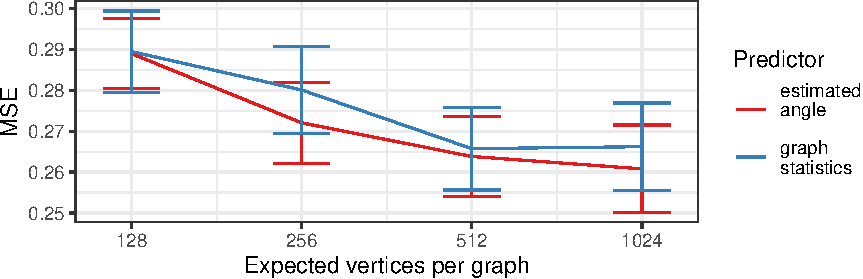
\includegraphics{draft_files/figure-latex/angle-regression-sim-1} 

}

\caption{The average MSE over 50 simulations in scenario 1. The errorbars are the standard error.}\label{fig:angle-regression-sim}
\end{figure}

\begin{figure}[H]

{\centering 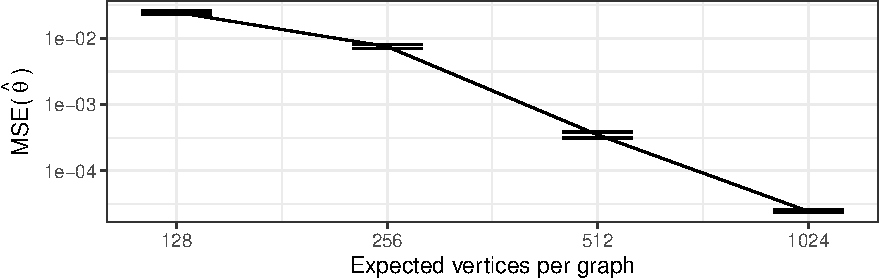
\includegraphics{draft_files/figure-latex/theta-mse-1} 

}

\caption{The average MSE of the estimated angles in scenario 1 over 50 simulations. The errorbars are the standard error.}\label{fig:theta-mse}
\end{figure}

\begin{figure}[H]

{\centering 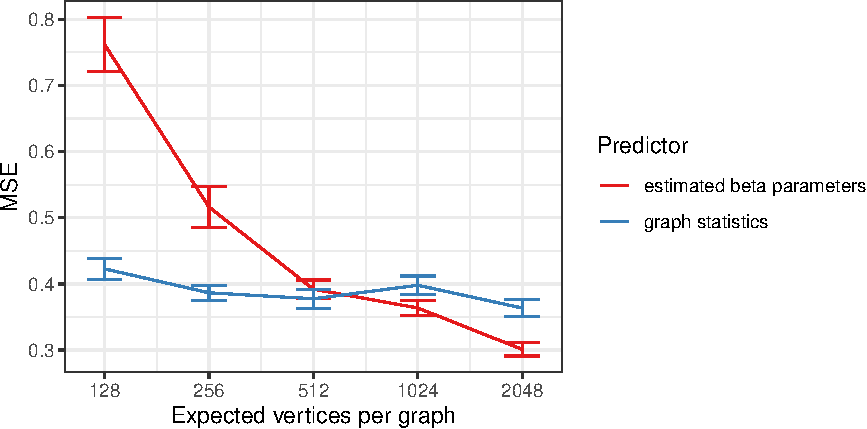
\includegraphics{draft_files/figure-latex/beta-regression-sim-1} 

}

\caption{The average MSE over 50 simulations in scenario 2. The errorbars are the standard error.}\label{fig:beta-regression-sim}
\end{figure}

\begin{figure}[H]

{\centering 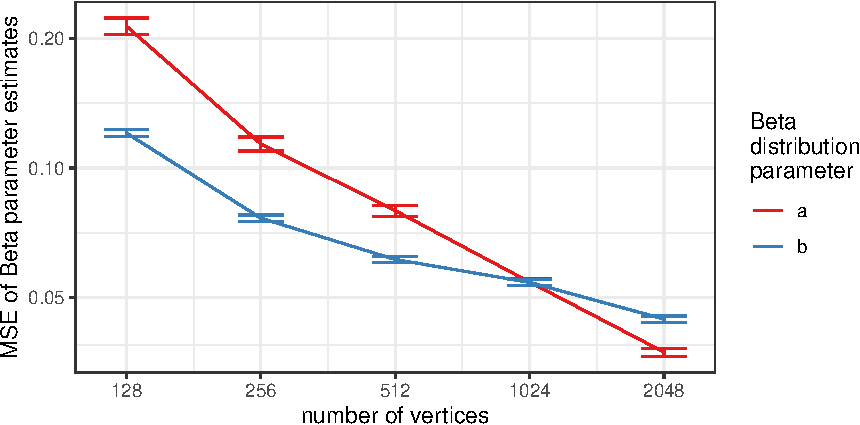
\includegraphics{draft_files/figure-latex/beta-mse-1} 

}

\caption{The average MSE of the estimated beta parameters, $(a, b)$, in scenario 2 over 50 simulations. The errorbars are the standard error.}\label{fig:beta-mse}
\end{figure}

\subsection{Classification}\label{classification}

In this simulation experiment, the latent vectors were sampled along a
Bezier curve defined by \(g(t) = \bigl[ t^2 \; 2 t (1-t) \bigr]^\top\).
The timepoints \(t_i\) were sampled as iid Beta random variables with
two sets of parameters, \((\alpha_1, \beta_1)\) and
\((\alpha_2, \beta_2)\). The setup is as follows:

\begin{enumerate}
\def\labelenumi{\arabic{enumi}.}
\tightlist
\item
  Draw response variables \(y_1, ..., y_n \iid \Multinomial(1/2, 1/2)\).
\item
  For each \(i = 1, ..., n\), draw
  \(t_i \mid y_i \indep \Betadist(\alpha_{y_i}, \beta_{y_i})\), such
  that \(\alpha_1 = 1\), \(\beta_1 = 2\), \(\alpha_2 = 2\), and
  \(\beta_2 = 1\).
\item
  Construct each latent vector as \(x_i = g(t_i)\) and compile them in
  data matrix \(X = \bigl[ x_1 \; \cdots \; x_n \bigr]^\top\).
\item
  Sample graph and its adjacency matrix as \(A \sim \RDPG(X)\).
\end{enumerate}

For each graph, we constructed the ASE, which was used to estimate the
parameters \((\hat{\alpha}, \hat{\beta})\) for the graph, using the
maximum likelihood method. The estimated parameters were then used as
predictors \(y_1, ..., y_n\), setting aside half for training and half
for testing. We investigated graphs of size \(|V| = 32, 64, 128, 256\).
The number of graphs for each experiment was set to \(L = 64\). For each
(number of graphs, size of graph) pair, we performed 32 replicates.
Figure \ref{fig:class-sim-ase} shows the ASE of one graph.\\
Figure \ref{fig:classification-sim} shows the boxplots of the
classification error rates.

\begin{figure}[H]

{\centering 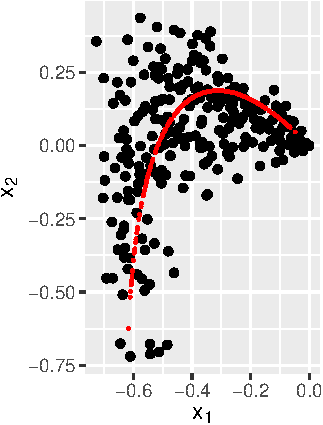
\includegraphics{draft_files/figure-latex/class-sim-ase-1} 

}

\caption{One simulated graph (left) and its ASE (right). The red curve is the fitted quadratic Bezier curve on the ASE.}\label{fig:class-sim-ase}
\end{figure}

\begin{figure}[H]

{\centering 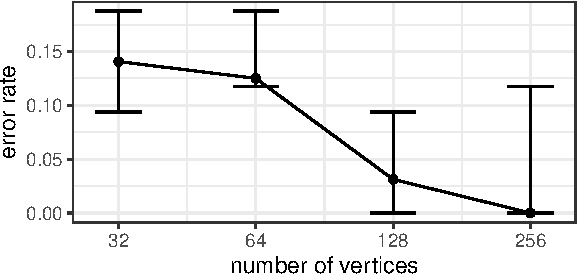
\includegraphics{draft_files/figure-latex/classification-sim-1} 

}

\caption{Median classification error rate and its IQR vs. number of vertices in each graph.}\label{fig:classification-sim}
\end{figure}

\subsection{Regression}\label{regression-1}

In the first regression simulation,

In the next regression simulation, we applied

\begin{enumerate}
\def\labelenumi{\arabic{enumi}.}
\tightlist
\item
  Draw angles
  \(\theta_1, ..., \theta_N \iid \Uniform(\pi / 6, \pi / 3)\).
\item
  For each \(k = 1, ..., N\),

  \begin{enumerate}
  \def\labelenumii{\roman{enumii}.}
  \tightlist
  \item
    Draw \(t_1, ..., t_n \iid \Uniform(0, 1)\);
  \item
    Draw \(z_1, ..., z_n \iid \Multinomial(1/2, 1/2)\);
  \item
    For each \(i = 1, ..., n\), set
    \(x_i = \begin{cases} \bigl[ t_i \; 0 \bigr]^\top \; z_i = 1 \\ \bigl[ t_i \cos \theta_\ell \; t_i \sin \theta_\ell \bigr]^\top \; z_i = 2 \end{cases}\);
  \item
    Collect \(X = \bigl[ x_1 \; \cdots \; x_n \bigr]^\top\) and draw
    \(A \sim \RDPG(X)\);
  \item
    Set the response \(y_\ell = \beta_0 + \beta_1 \theta_\ell\)
  \end{enumerate}
\end{enumerate}

In this simulation, we set \(\beta_0 = \beta_1 = 1\). The number of
graphs was set to \(L = 64\), and the number of vertices per graph was
set to \(n = 128, 256, 512, 1024\). For each \(n\), we simulated 32
replicates.

\begin{center}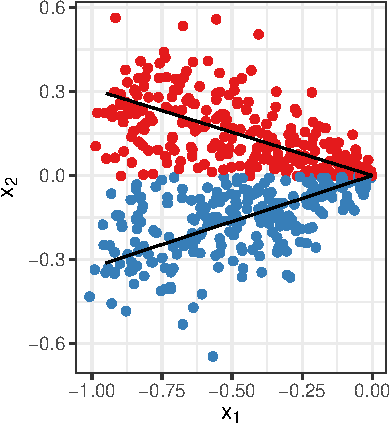
\includegraphics{draft_files/figure-latex/angle-reg-example-1} \end{center}

\begin{center}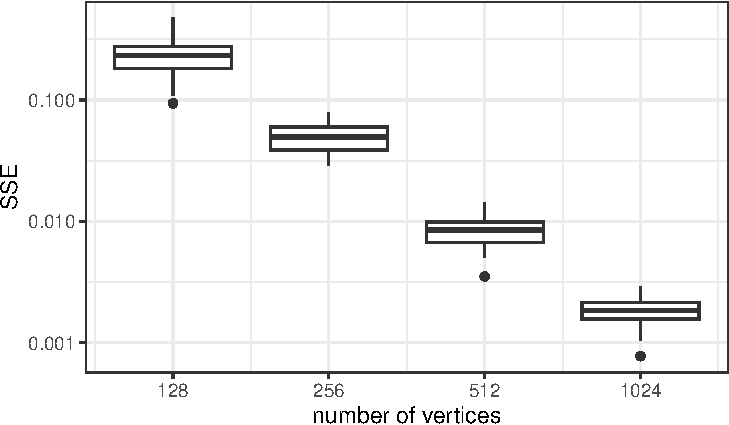
\includegraphics{draft_files/figure-latex/angle-reg-results-1} \end{center}

\section{Applications}\label{applications}

\subsection{Drosophila Connectome}\label{drosophila-connectome}

In the second example, we analyzed the larval \emph{Drosophila} mushroom
body connectome \citep{Eichler141762}, which has been studied as a GRDPG
by \citet{athreya2020estimation}. This dataset consists of two graphs
representing two networks of neurons, one for each hemisphere of the
\emph{Drosophila} brain. In these graphs, each vertex is a neuron, and
the labels correspond to one of four neuron types (Kenyon Cells, Input
Neurons, Output Neurons, and Projection Neurons). The number of neurons
in each hemisphere is not equal (209 in the left hemisphere and 213 in
the right hemisphere). The resulting graphs are illustrated in figure
\ref{fig:mbconnectome-graph}.

\begin{figure}[H]

{\centering \includegraphics{draft_files/figure-latex/mbconnectome-graph-1} 

}

\caption{Graphs of the Drosophila connectomes. The left and right are of the left and right hemispheres, respectively. Each vertex represents a neuron, which are labeled by neuron type.}\label{fig:mbconnectome-graph}
\end{figure}

\begin{figure}[H]

{\centering 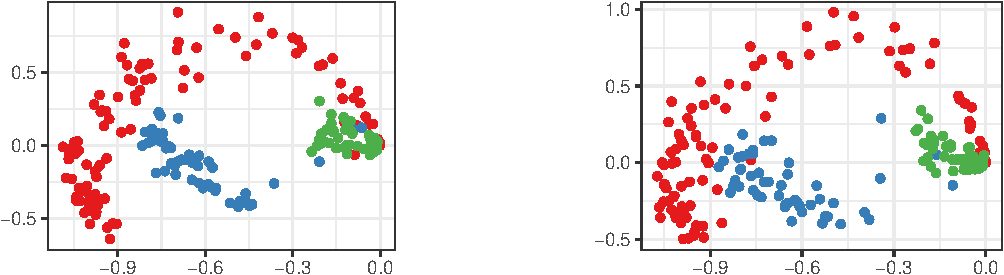
\includegraphics{draft_files/figure-latex/mbconnectome-ase-1} 

}

\caption{ASEs of the Drosophila connectome graphs. The embedding vectors are labeled by neuron type. }\label{fig:mbconnectome-ase}
\end{figure}

When analyzed as a GRDPG, the ASE of each hemisphere suggests that nodes
of each type falls along a curve in the latent space (figure
\ref{fig:mbconnectome-ase}). In our analysis, we set the embedding
dimension to \(d = 4\), with 3 assortative dimensions and 1
disassortative dimension, and the figure only shows the first two
assortative dimensions. This matches observations by
\citet{athreya2020estimation}. We fit three latent structure Bezier
curves, one for Kenyon Cells, one for Input and Output Neurons, and one
for Projection Neurons, to the embedding for each hemisphere. Then we
fit a Beta distribution to to the timepoints along each curve and
extracted the two Beta parameter estimates (via likelihood maximization)
for each curve. If these Beta parameters are informative, we would
expect the parameters for each hemisphere to match by neuron type, which
is what we observe in these data (fig \ref{fig:mbconnectome-beta}).
Using the three subgraphs of the left hemisphere as a training set to
classify which subgraph of the right hemisphere belongs to which neuron
type using the extracted Beta distribution parameter estimates as
predictors results in 100\% accuracy.

\begin{figure}[H]

{\centering 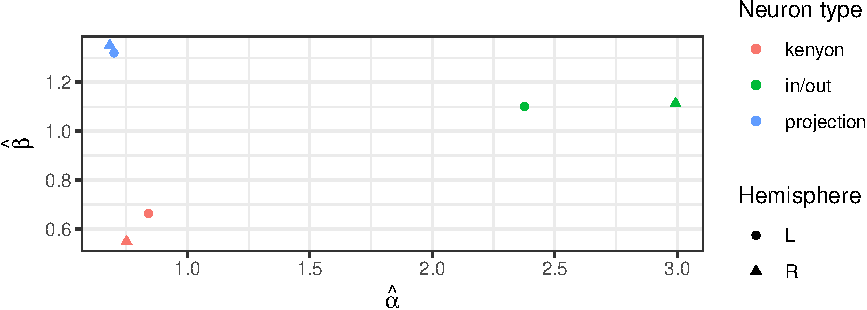
\includegraphics{draft_files/figure-latex/mbconnectome-beta-1} 

}

\caption{Beta parameter estimates for each curve and hemisphere.}\label{fig:mbconnectome-beta}
\end{figure}

\subsection{Human Connectome Project Aging
Study}\label{human-connectome-project-aging-study}

In the second example, we analyzed fiber count data between brain
regions from the Human Connectome Project (HCP). When analyzing these
data as graphs, we denote the regions as vertices and the fiber counts
between pairs of regions as weighted edges. A plausible statistical
model for these data is to assume that the edge weights between pairs of
vertices is Poisson distributed, i.e., the adjacency matrix is sampled
as \(A_{ij} \indep \Poisson(\Theta_{ij})\), where
\(\Theta \in \mathbb{R}_+^{n \times n}\) is a symmetric matrix of
Poisson parameters.

In this dataset, there are \(L = 516\) graphs (corresponding to
individual subjects), each with \(n_\ell = n = 84\) vertices
(corresponding to brain regions). Analyzing these graphs as RDPGs
reveals that the DCBM is a good candidate for these data (figure
\ref{fig:hcp-ase}).

\begin{figure}[H]

{\centering 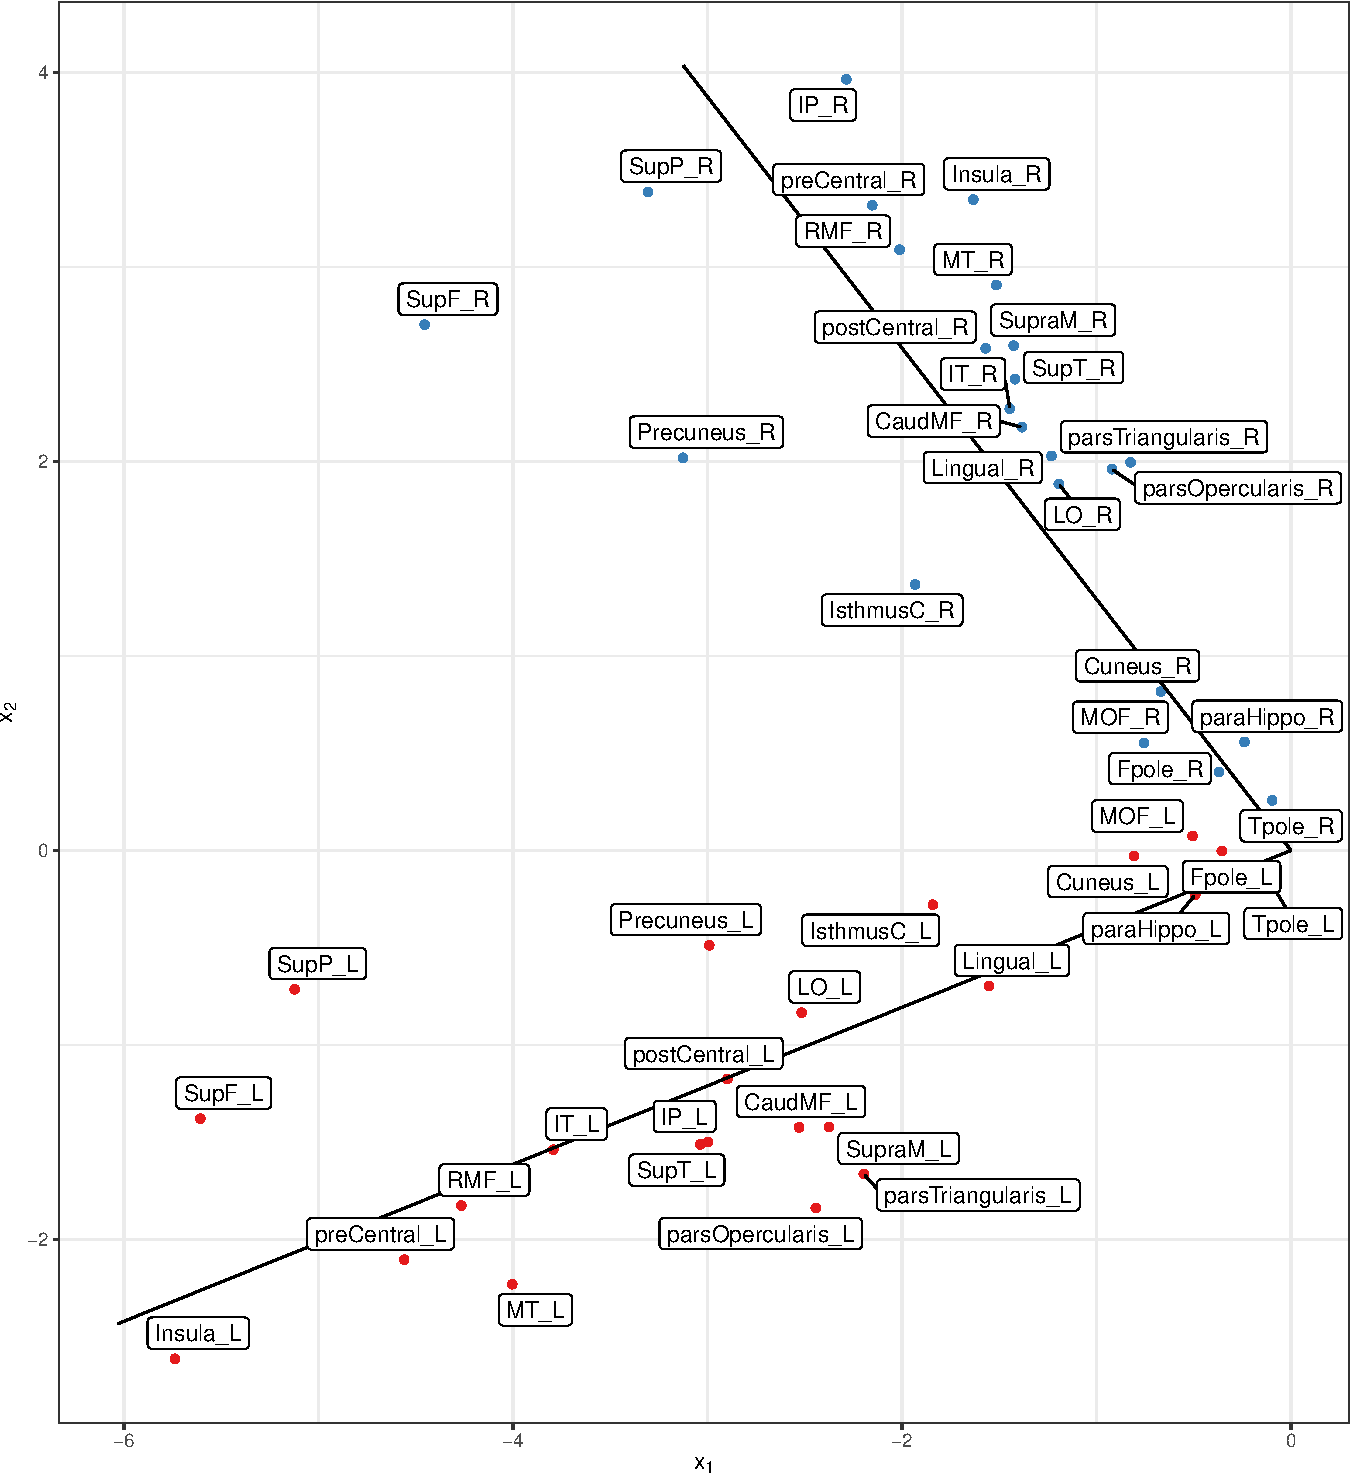
\includegraphics[width=1\linewidth]{draft_files/figure-latex/hcp-ase-1} 

}

\caption{One graph from the HCP dataset (left) and its ASE (right). In the ASE, the lines are fitted via $K$-curves clustering using degree = 1. The outputted clusters correspond exactly to the left (red) and right (blue) hemispheres.}\label{fig:hcp-ase}
\end{figure}

\begin{figure}[H]

{\centering 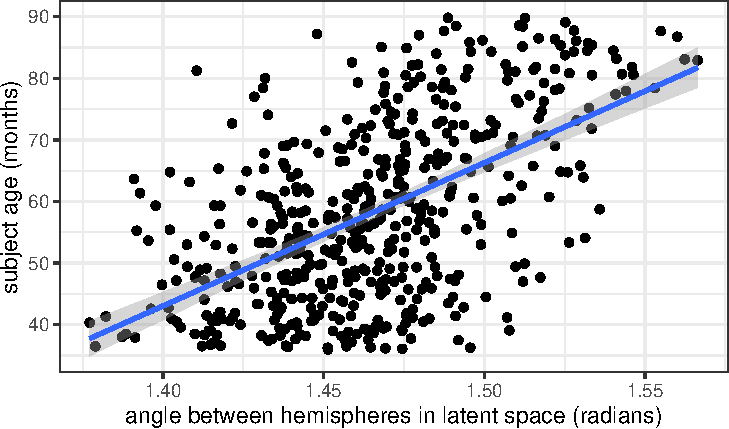
\includegraphics{draft_files/figure-latex/hcp-age-regression-1} 

}

\caption{Scatterplot between the subject age (in months) vs. the fitted angle between hemispheres of the brain in the latent space.}\label{fig:hcp-age-regression}
\end{figure}

The ASE suggests a latent structure comprised of two Bezier curves of
degree 1 (i.e., lines), one for each hemisphere of the brain, that meet
at the origin. One possible parameter when analyzing these data as a
MLSM is the angle between the two lines. The estimated angles were
observed to correlate with the subject's age, with wider angles
corresponding to older subjects (figure \ref{fig:hcp-age-regression}). A
linear regression setting aside half of the brain connectivity graphs as
test data achieves an RMSE of \(11.889\) months.

To compare this parameter as a covariate for age against other network
statistics, we analyzed these data as a multilayer DCBM, first studied
by \citep{agterberg2022joint}, who proposed the degree corrected
multiple adjacency spectral embedding (DC-MASE) algorithm. Since these
graphs come with hemisphere labels, we did not apply DC-MASE for
community detection but instead used the estimators for the three edge
connectivity parameters, \(B_{LL}\), \(B_{RR}\), and \(B_{LR}\). A
linear model trained on these parameter estimates achieves a higher RMSE
of \(12.889\) months, despite using three covariates instead of one. In
addition, since the angles between the latent structures under the MLSM
depend primarily on the shape of the latent structures rather than the
exact community memberships, it does not depend on recovery of the
original community labels. Ultimately, these two methods are estimators
for transformations of the same parameters, and while we cannot
determine how close these estimates are on the ``true'' edge
connectivity parameters since they are unknown, we observe that the MLSM
estimate is a better linear predictor than the rest.

Other graph statistics were extracted for each brain network, and their
correlations to age are reported in table \ref{tab:cor-comparison}. Note
that aside from the angle between the latent structures under the MLSM
model, these statistics assume that it is known which vertex belongs to
which hemisphere.

\begin{longtable}[]{@{}lrl@{}}
\caption{Correlation between age and various graph
metrics.\label{tab:cor-comparison}}\tabularnewline
\toprule\noalign{}
Metric & Correlation & 95\% conf. int. \\
\midrule\noalign{}
\endfirsthead
\toprule\noalign{}
Metric & Correlation & 95\% conf. int. \\
\midrule\noalign{}
\endhead
\bottomrule\noalign{}
\endlastfoot
Angle between hemispheres & 0.558 & (0.496, 0.615) \\
Degree within hemisphere & 0.436 & (0.363, 0.503) \\
Degree between hemispheres & -0.499 & (-0.561, -0.431) \\
Modularity w.r.t. hemisphere & 0.434 & (0.362, 0.502) \\
Joint Embedding & 0.556 & (0.493, 0.613) \\
\end{longtable}

Next, we considered each hemisphere separately and fit a Beta
distribution to the embedding of each half-network. The scatterplot of
the fitted \(\alpha\) and \(\beta\) parameters suggests that there are
two clusters of brain networks (figure \ref{fig:hcp-clustering}).
Greater \(\alpha\) values correspond to more embedding vectors farther
away from the origin, corresponding to more nodes of higher degree,
which in turn correspond to more brain regions with a greater number of
connections. Conversely, greater \(\beta\) values correspond to more
embedding vectors closer to the origin, which in turn correspond to more
brain regions with fewer connections. This may suggest that there are
underlying groups, one of which tends to have higher connectivity in the
left hemisphere, and the other having higher connectivity in the right
hemisphere.

\begin{figure}[H]

{\centering 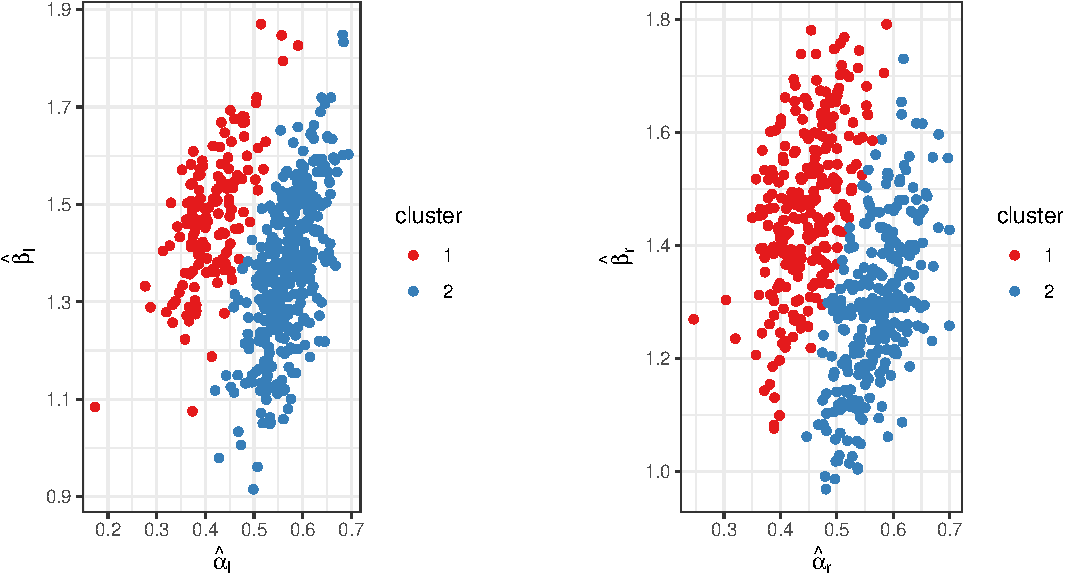
\includegraphics{draft_files/figure-latex/hcp-clustering-1} 

}

\caption{Scatterplot of fitted parameters of the Beta distribution. The left image are the parameters fitted on the embedding of the left hemisphere, and the right image are the parameters fitted on the embedding of the right hemisphere.}\label{fig:hcp-clustering}
\end{figure}

\section{Discussion}\label{discussion}

\section*{Appendix A: Proofs of Theorems}

\newpage

\bibliographystyle{apalike}
\renewcommand\refname{Bibliography}
\bibliography{bibliography.bib}



\end{document}
